\chapter{IMPLEMENTATION}

\section{Technology Stack}
The implementation of the CRM System leverages the MERN technology stack, incorporating modern industry frameworks, build tools, and software engineering libraries:
\begin{itemize}
    \item \textbf{Frontend:} React.js (v18.2.0) configured with Vite (v5.2.8) for fast module replacement, Tailwind CSS (v3.4.3) for styling, React Router DOM (v6.22.3) for single-page routing, Axios (v1.6.8) for HTTP networking, Lucide React (v0.364.0) for accessible icons, and Recharts (v2.12.3) for dynamic data visualization.
    \item \textbf{Backend:} Node.js (v20+ LTS) and Express.js (v4.19.2), structured as a REST API architecture utilizing JSON Web Tokens (\texttt{jsonwebtoken} v9.0.2) for stateless authentication, \texttt{bcryptjs} (v2.4.3) for cryptographic salt-and-hash operations, \texttt{cors} (v2.8.5) for cross-origin security, and \texttt{morgan} (v1.10.0) for HTTP transaction logging.
    \item \textbf{Database:} MongoDB Atlas cloud cluster connected through Mongoose ODM (v8.3.1), utilizing asynchronous connection pooling, schema validations, pre-save middleware hooks, relational document population, and multi-stage aggregation pipelines.
\end{itemize}

\section{Frontend Implementation}
The client application is built as an ergonomic Single Page Application (SPA). Global authentication state is managed via \texttt{AuthContext.jsx}, storing the active user profile and token in browser \texttt{localStorage} to ensure session persistence across browser reloads. Centralized Axios interceptors in \texttt{axiosClient.js} automatically inject the authorization bearer header into outgoing requests:

\begin{lstlisting}[language=JavaScript, caption={Axios Client Interceptors in \texttt{frontend/src/api/axiosClient.js}}]
import axios from 'axios';

const API_BASE_URL = import.meta.env.VITE_API_URL || '/api/v1';

const axiosClient = axios.create({
  baseURL: API_BASE_URL,
  headers: { 'Content-Type': 'application/json' }
});

// Request interceptor to attach JWT token
axiosClient.interceptors.request.use((config) => {
  const token = localStorage.getItem('crm_token');
  if (token) {
    config.headers.Authorization = `Bearer ${token}`;
  }
  return config;
});

// Response interceptor to handle unauthorized 401 errors
axiosClient.interceptors.response.use(
  (response) => response.data,
  (error) => {
    if (error.response && error.response.status === 401) {
      localStorage.removeItem('crm_token');
      localStorage.removeItem('crm_user');
      if (window.location.pathname !== '/login') {
        window.location.href = '/login?expired=true';
      }
    }
    return Promise.reject(new Error(error.response?.data?.message || 'Error'));
  }
);
\end{lstlisting}

\section{React Application Structure}
The frontend source code is organized into modular folders under \texttt{frontend/src/}:
\begin{itemize}
    \item \texttt{api/}: Centralized Axios client instance and endpoint constants.
    \item \texttt{components/}:
    \begin{itemize}
        \item \texttt{auth/}: \texttt{ProtectedRoute.jsx} protecting private routes by role.
        \item \texttt{common/}: Reusable UI widgets (\texttt{Badge.jsx}, \texttt{Modal.jsx}, \texttt{Pagination.jsx}, \texttt{ConfirmDialog.jsx}, \texttt{LoadingSkeleton.jsx}, \texttt{EmptyState.jsx}).
        \item \texttt{layout/}: Application frame consisting of \texttt{DashboardLayout.jsx}, \texttt{Sidebar.jsx}, and \texttt{TopNavbar.jsx}.
    \end{itemize}
    \item \texttt{context/}: \texttt{AuthContext.jsx} (state, login, logout, profile updates) and \texttt{ToastContext.jsx} (toast alerts).
    \item \texttt{pages/}: The twelve operational screen components.
\end{itemize}

\section{Login Page Implementation}
The \texttt{Login.jsx} component delivers an intuitive authentication portal. It provides direct single-click credential quick-fill cards for all four system roles (\textit{Admin, Sales Manager, Sales Executive, Customer Support}), an automated demo password fill mechanism, a remember-session checkbox, a password visibility toggle, and client-side form validation. Invalid credentials trigger red feedback alerts without corrupting browser state.

\begin{figure}[h!]
\centering
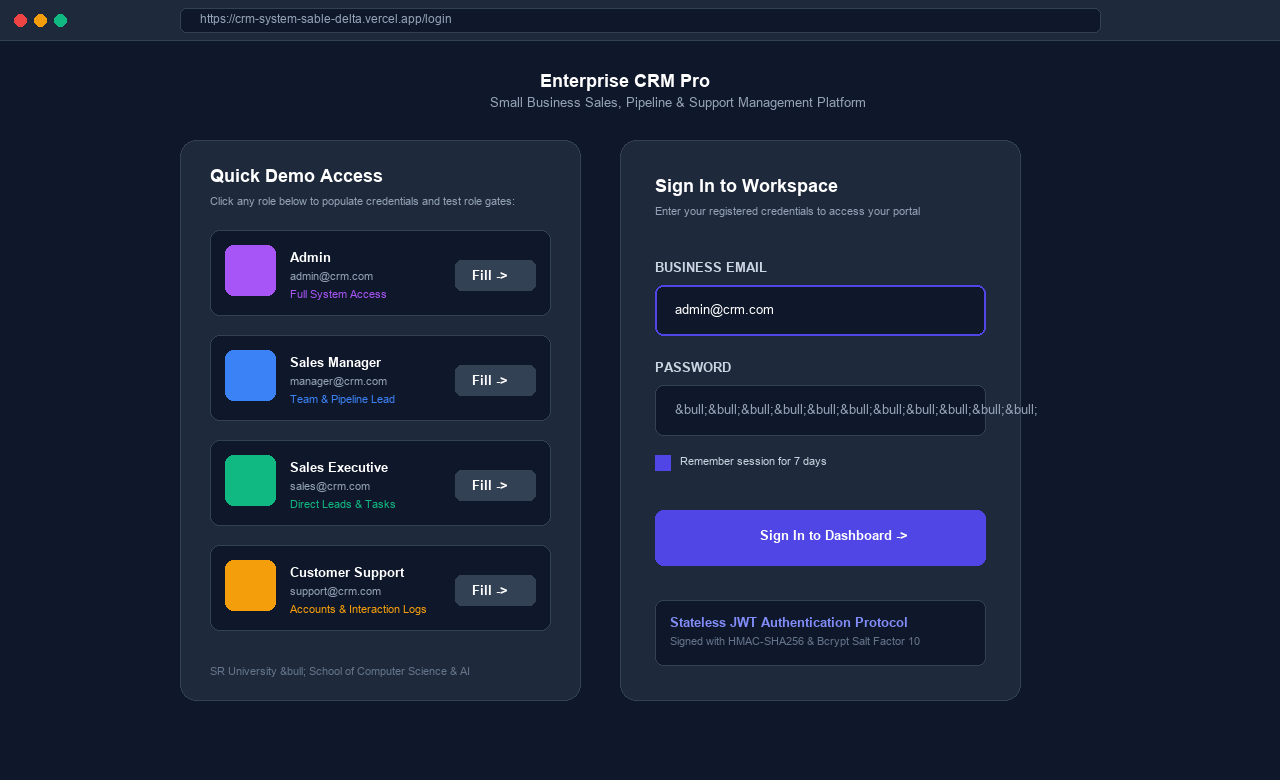
\includegraphics[width=0.95\textwidth]{figures/screen_login.png}
\caption{CRM Portal Authentication Interface with Multi-Role Demo Cards}
\label{fig:screen_login}
\end{figure}

\section{Dashboard Implementation}
The \texttt{Dashboard.jsx} screen acts as the operational nerve center. Upon mounting, it dispatches an asynchronous call to \texttt{/api/v1/dashboard}, retrieving:
\begin{enumerate}
    \item \textbf{KPI Summary Cards:} Total Customers, Active Leads in Pipeline, Closed Won Revenue, and Pending Follow-ups with percentage trend indicators.
    \item \textbf{Monthly Revenue Analytics:} An interactive Recharts area/bar chart displaying twelve-month revenue trends.
    \item \textbf{Lead Source Breakdown:} A Recharts pie chart categorizing lead acquisition channels (Website, Referrals, LinkedIn, Cold Calls).
    \item \textbf{Recent Activity Feeds:} Tabular widgets displaying recently logged interactions, impending tasks, and high-value opportunities.
\end{enumerate}

\begin{figure}[h!]
\centering
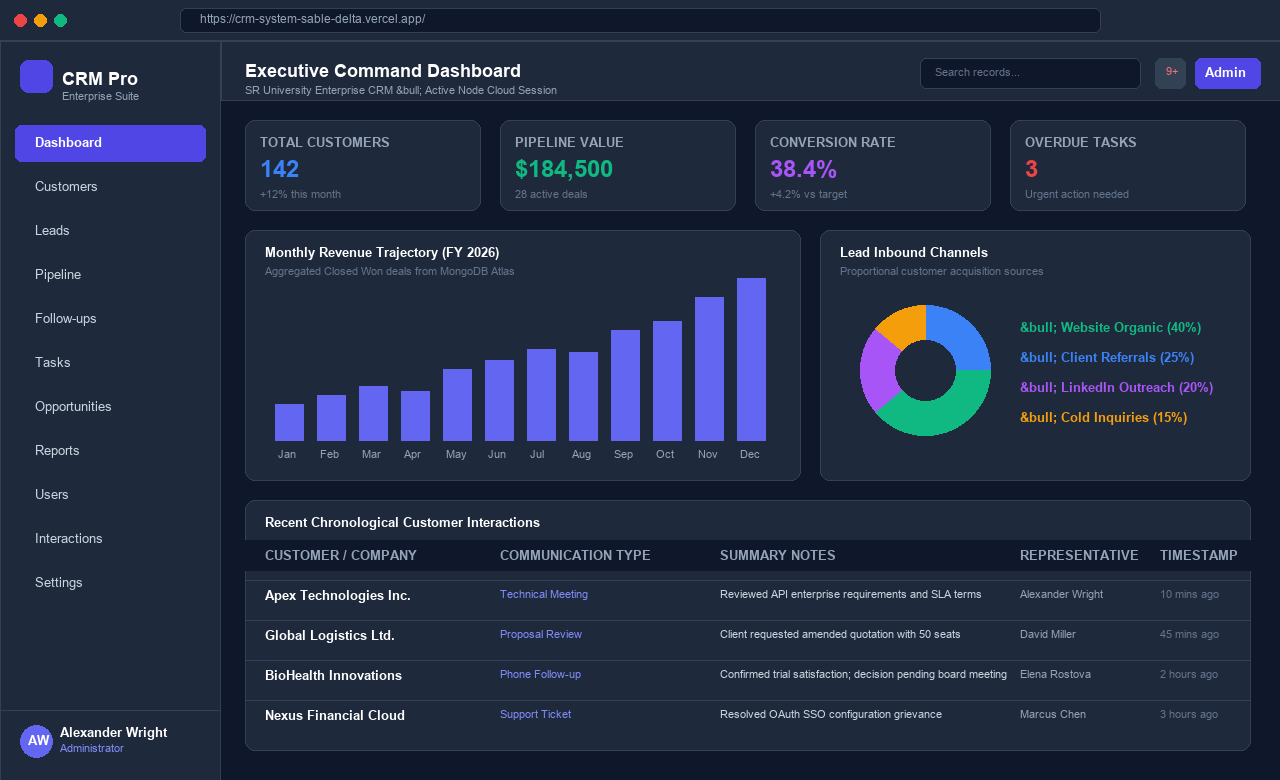
\includegraphics[width=0.95\textwidth]{figures/screen_dashboard.png}
\caption{Executive Command Dashboard Featuring Real-Time KPIs and Recharts Analytics}
\label{fig:screen_dashboard}
\end{figure}

\section{Customer Management Module}
The \texttt{Customers.jsx} page provides end-to-end account management. Users can search by customer name, company, or email, filter by account status (\textit{Lead, Active, Inactive}), and sort columns dynamically. Clicking ``Add Customer'' launches an accessible modal dialog containing field validations. Editing updates records via \texttt{PUT /api/v1/customers/:id}, and deletion triggers a secondary confirmation modal.

\begin{figure}[h!]
\centering
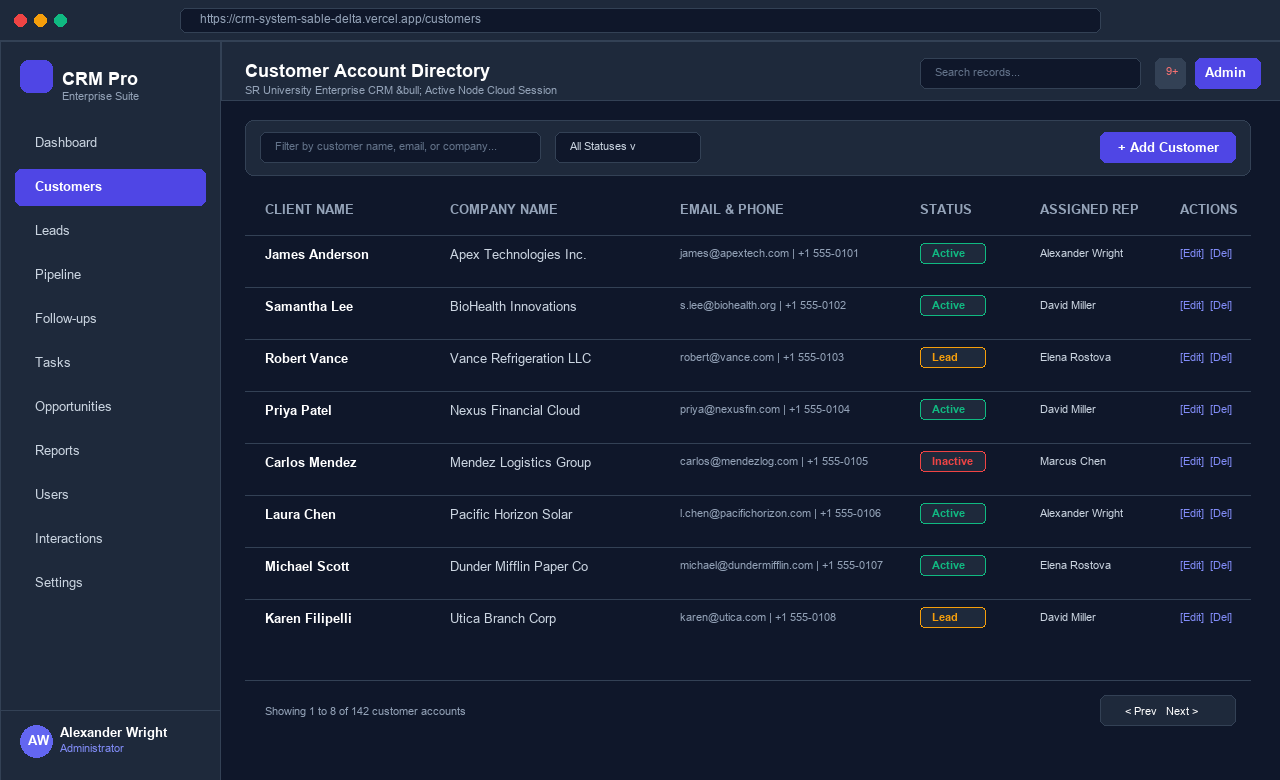
\includegraphics[width=0.95\textwidth]{figures/screen_customers.png}
\caption{Customer Account Management Directory with Multi-Criteria Search and Filtering}
\label{fig:screen_customers}
\end{figure}

\section{Lead Management Module}
The \texttt{Leads.jsx} module coordinates prospect ingestion and qualification. Each lead record captures the contact individual, company, lead source, assigned sales executive, estimated deal value, and priority score. A dedicated ``Convert to Customer'' action allows sales representatives to transition qualified prospects directly into the customer registry, automatically instantiating a connected customer record and closing the lead with zero data re-entry.

\begin{figure}[h!]
\centering
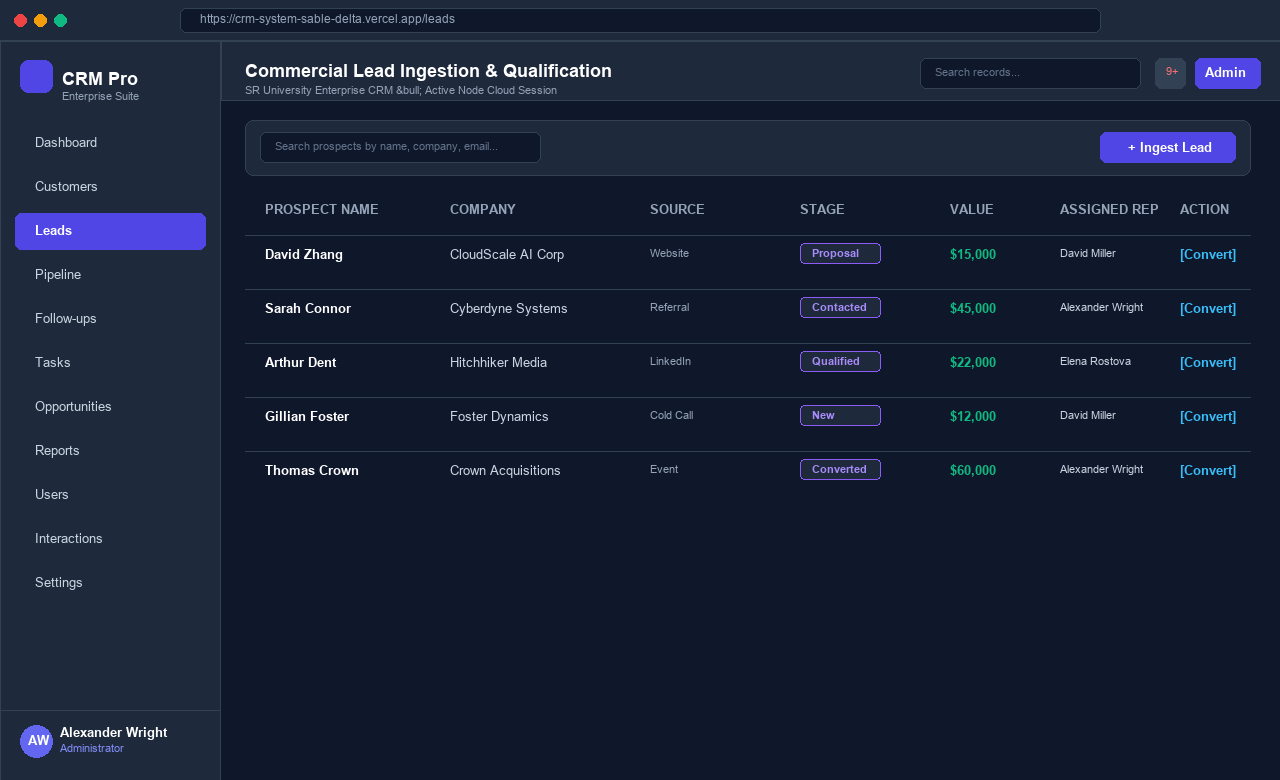
\includegraphics[width=0.95\textwidth]{figures/screen_leads.png}
\caption{Commercial Lead Ingestion, Qualification, and Conversion Module}
\label{fig:screen_leads}
\end{figure}

\section{Task Management Module}
The \texttt{Tasks.jsx} module organizes operational workflows. Tasks are categorized by priority level (\textit{Urgent, High, Medium, Low}) and status (\textit{Pending, In Progress, Completed, Deferred}). Visual badge indicators highlight overdue tasks whose deadlines have elapsed, and direct completion checkboxes trigger non-blocking API status updates.

\begin{figure}[h!]
\centering
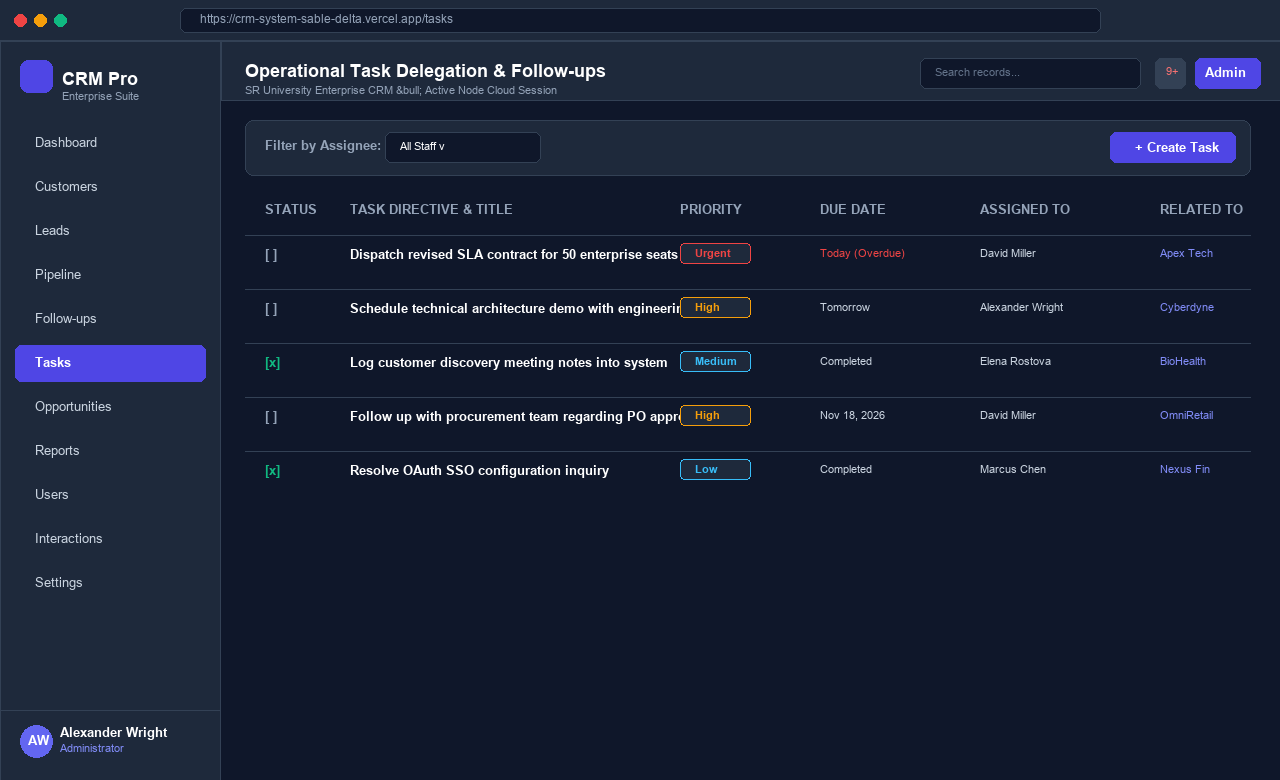
\includegraphics[width=0.95\textwidth]{figures/screen_tasks.png}
\caption{Operational Task Delegation Board with Priority Badges and Deadline Tracking}
\label{fig:screen_tasks}
\end{figure}

\section{Visual Kanban Pipeline & Reporting Implementation}
The system delivers an interactive Kanban sales pipeline (\texttt{SalesPipeline.jsx}) allowing dynamic deal stage updates, and a comprehensive reporting suite (\texttt{Reports.jsx}) backed by MongoDB aggregations.

\begin{figure}[h!]
\centering
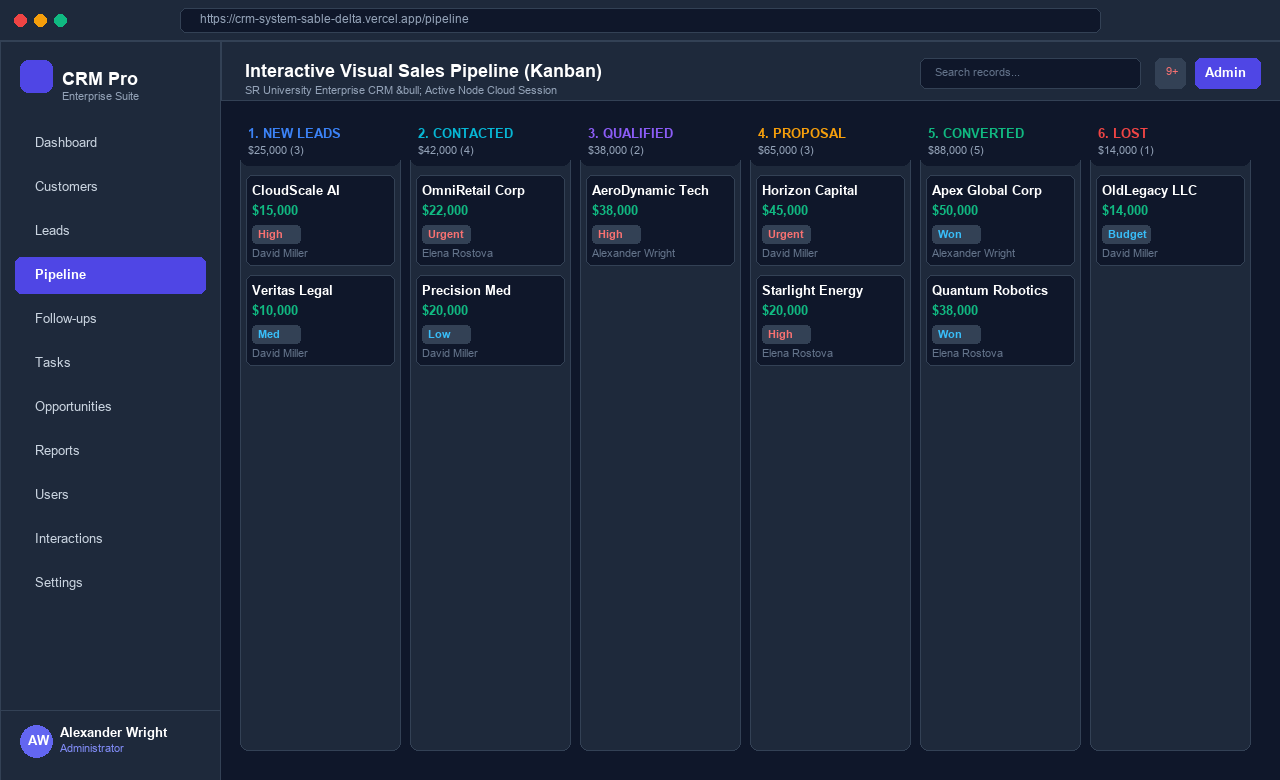
\includegraphics[width=0.95\textwidth]{figures/screen_pipeline.png}
\caption{Interactive Kanban Sales Pipeline with Six Stage-Gate Deal Columns}
\label{fig:screen_pipeline}
\end{figure}

\begin{figure}[h!]
\centering
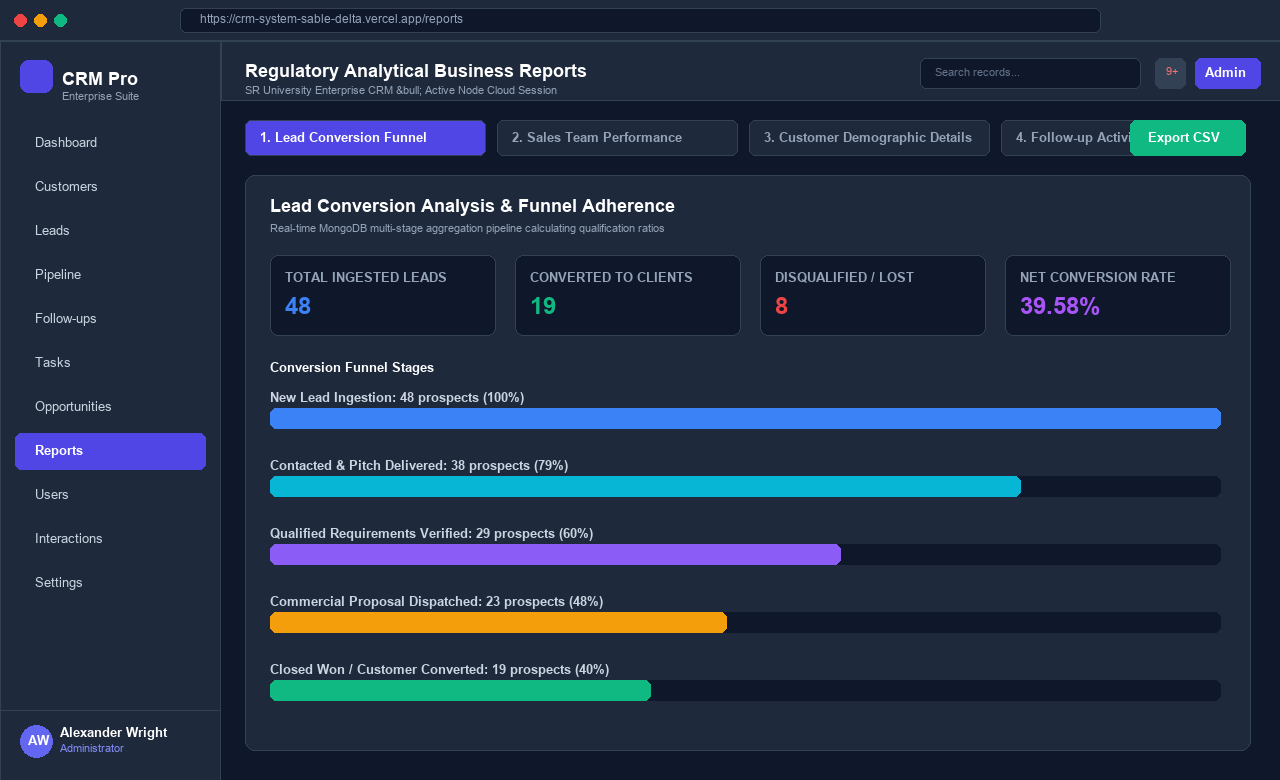
\includegraphics[width=0.95\textwidth]{figures/screen_reports.png}
\caption{Mandatory Analytical Reports Suite with Real-Time Conversion Funnel and CSV Export}
\label{fig:screen_reports}
\end{figure}

\begin{figure}[h!]
\centering
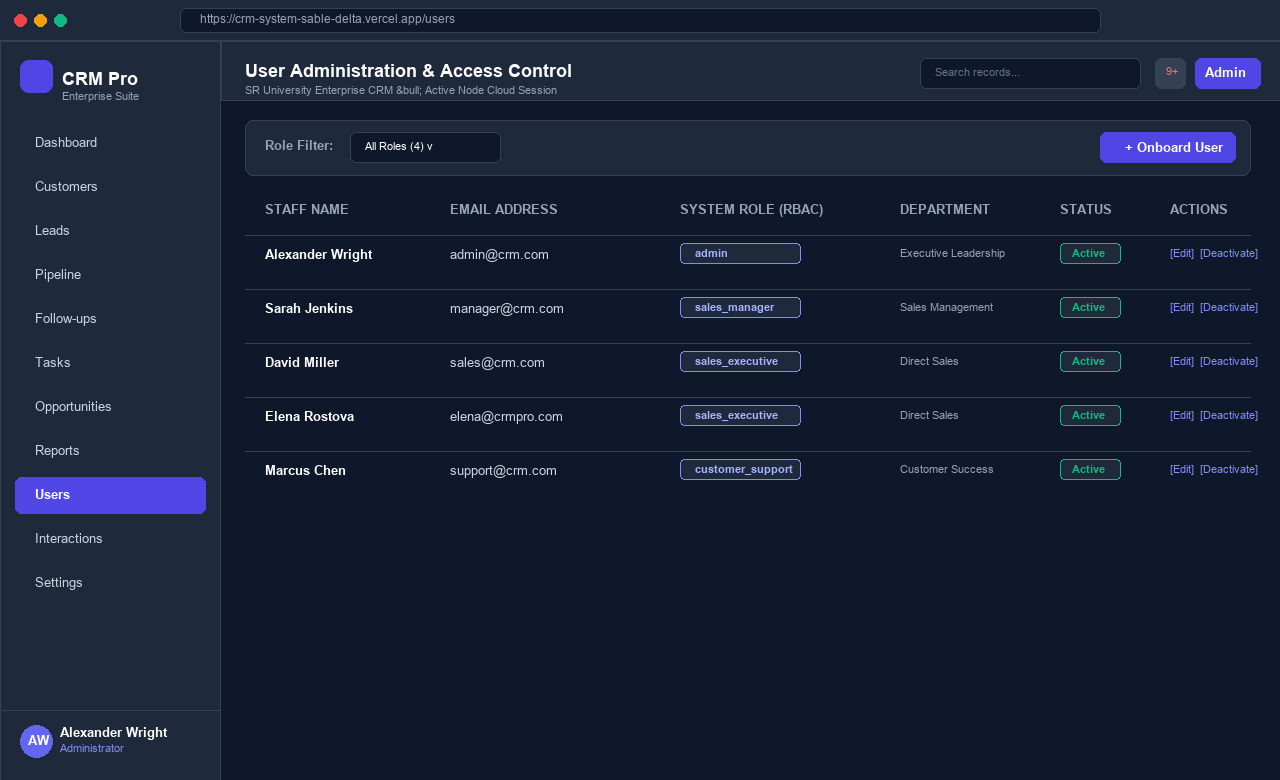
\includegraphics[width=0.95\textwidth]{figures/screen_users.png}
\caption{User Administration Console with Role-Based Access Control Boundaries}
\label{fig:screen_users}
\end{figure}

\section{Backend Implementation}
The backend server is implemented as an asynchronous Node.js Express service. In \texttt{server.js}, incoming requests are processed through body parsers, CORS handlers, route mappers, and an error interception pipeline. When starting up, the server invokes \texttt{connectDB()} to verify MongoDB Atlas connectivity, followed by an automatic bootstrap check: if the database has zero user records, the automated seeder (\texttt{seeder.js}) populates the cluster with system users, realistic customers, pipeline leads, and sample transactions.

\section{REST API Implementation}
Table~\ref{tab:api_endpoints} documents the complete REST API endpoints implemented across the eleven backend route controllers.

\begin{table}[h!]
\centering
\caption{Complete Backend REST API Route Specification}
\label{tab:api_endpoints}
\renewcommand{\arraystretch}{1.2}
\begin{tabular}{|p{1.5cm}|p{5.5cm}|p{3.5cm}|p{4cm}|}
\hline
\textbf{Verb} & \textbf{Endpoint Route} & \textbf{Authorized Roles} & \textbf{Description} \\ \hline
\texttt{GET} & \texttt{/health} & Public & Cloud uptime health check probe \\ \hline
\texttt{POST} & \texttt{/api/v1/auth/login} & Public & Authenticates user; returns JWT \\ \hline
\texttt{GET} & \texttt{/api/v1/auth/me} & All Authenticated & Retrieves active user session profile \\ \hline
\texttt{PUT} & \texttt{/api/v1/auth/updateprofile} & All Authenticated & Updates user name, phone, dept \\ \hline
\texttt{PUT} & \texttt{/api/v1/auth/updatepassword} & All Authenticated & Validates current and sets new password \\ \hline
\texttt{GET} & \texttt{/api/v1/dashboard} & All Authenticated & Computes KPIs and chart analytics \\ \hline
\texttt{GET} & \texttt{/api/v1/customers} & All Authenticated & Lists customers with search/pagination \\ \hline
\texttt{POST} & \texttt{/api/v1/customers} & Admin, Manager, Exec & Creates new customer record \\ \hline
\texttt{GET} & \texttt{/api/v1/customers/:id} & All Authenticated & Retrieves single customer details \\ \hline
\texttt{PUT} & \texttt{/api/v1/customers/:id} & Admin, Manager, Exec & Updates customer account profile \\ \hline
\texttt{DELETE}& \texttt{/api/v1/customers/:id} & Admin Only & Permanently deletes customer \\ \hline
\texttt{GET} & \texttt{/api/v1/leads} & Admin, Manager, Exec & Retrieves leads with stage filters \\ \hline
\texttt{POST} & \texttt{/api/v1/leads} & Admin, Manager, Exec & Ingests new commercial lead \\ \hline
\texttt{PUT} & \texttt{/api/v1/leads/:id} & Admin, Manager, Exec & Updates lead information/notes \\ \hline
\texttt{DELETE}& \texttt{/api/v1/leads/:id} & Admin, Manager & Removes lead record \\ \hline
\texttt{POST} & \texttt{/api/v1/leads/:id/convert} & Admin, Manager, Exec & Converts lead into verified customer \\ \hline
\texttt{GET} & \texttt{/api/v1/pipeline} & Admin, Manager, Exec & Groups active deals into Kanban stages \\ \hline
\texttt{PUT} & \texttt{/api/v1/pipeline/stage/:id}& Admin, Manager, Exec & Updates stage of lead in pipeline \\ \hline
\texttt{GET} & \texttt{/api/v1/opportunities} & Admin, Manager, Exec & Lists commercial opportunities \\ \hline
\texttt{POST} & \texttt{/api/v1/opportunities} & Admin, Manager, Exec & Creates new revenue opportunity \\ \hline
\texttt{GET} & \texttt{/api/v1/tasks} & All Authenticated & Lists tasks assigned to users \\ \hline
\texttt{POST} & \texttt{/api/v1/tasks} & Admin, Manager, Exec & Delegates task to employee \\ \hline
\texttt{PUT} & \texttt{/api/v1/tasks/:id} & All Authenticated & Toggles status or updates task \\ \hline
\texttt{GET} & \texttt{/api/v1/followups} & All Authenticated & Lists scheduled follow-up activities \\ \hline
\texttt{POST} & \texttt{/api/v1/followups} & Admin, Manager, Exec & Schedules client callback or meeting \\ \hline
\texttt{GET} & \texttt{/api/v1/interactions} & All Authenticated & Retrieves chronological client logs \\ \hline
\texttt{POST} & \texttt{/api/v1/interactions} & All Authenticated & Logs new phone call, note, or meeting \\ \hline
\texttt{GET} & \texttt{/api/v1/reports/lead-conversion} & Admin, Manager & Lead conversion rate funnel \\ \hline
\texttt{GET} & \texttt{/api/v1/reports/sales-performance}& Admin, Manager & Rep-wise revenue and won deals \\ \hline
\texttt{GET} & \texttt{/api/v1/reports/customer-details} & Admin, Manager & Customer account demographic report \\ \hline
\texttt{GET} & \texttt{/api/v1/reports/followup-activity} & Admin, Manager & Follow-up adherence analysis \\ \hline
\texttt{GET} & \texttt{/api/v1/users} & Admin Only & Lists all employee user accounts \\ \hline
\texttt{POST} & \texttt{/api/v1/users} & Admin Only & Onboards new employee account \\ \hline
\texttt{PUT} & \texttt{/api/v1/users/:id} & Admin Only & Modifies role or account status \\ \hline
\end{tabular}
\end{table}

\section{MongoDB Database Implementation}
Database connectivity is managed in \texttt{backend/src/config/db.js} using Mongoose with a connection pooling pool size of 10. The connection logic implements a robust fallback strategy: it first attempts to connect to the cloud \texttt{MONGO\_URI}; if in a development setting where no remote database is supplied, it spins up an embedded in-memory MongoDB instance to ensure uninterrupted development.

\section{Authentication Implementation}
User authentication utilizes industry-standard JSON Web Tokens (RFC 7519)~\cite{rfc7519jwt}. During login, the server retrieves the user document, performs constant-time bcrypt password comparison, and signs a token:
\begin{equation}
\text{JWT} = \text{HMAC-SHA256}\Big(\text{Base64Url}(\text{Header}) \,||\, \text{Base64Url}(\text{Payload}), \, \text{JWT\_SECRET}\Big)
\end{equation}
The signed payload contains the user's MongoDB \texttt{\_id} and \texttt{role}, serialized with a 7-day expiration time (\texttt{JWT\_EXPIRES\_IN: '7d'}).

\section{Authorization and Security}
Authorization is strictly enforced on both tiers. The server middleware \texttt{auth.js} extracts and verifies the bearer token from the HTTP headers, binding the authenticated user document to \texttt{req.user}. The \texttt{rbac.js} middleware intercepts unauthorized requests:

\begin{lstlisting}[language=JavaScript, caption={Server RBAC Authorization Middleware in \texttt{backend/src/middleware/rbac.js}}]
const authorize = (...roles) => {
  return (req, res, next) => {
    if (!req.user || !roles.includes(req.user.role)) {
      return res.status(403).json({
        success: false,
        message: `User role '${req.user?.role}' is unauthorized to access this resource`
      });
    }
    next();
  };
};
module.exports = { authorize };
\end{lstlisting}

\section{CRUD Operations}
All primary entities (\texttt{Customer}, \texttt{Lead}, \texttt{Opportunity}, \texttt{Task}, \texttt{FollowUp}, \texttt{Interaction}, \texttt{User}) feature atomic CRUD database handlers. Controller functions employ Mongoose helper methods such as \texttt{.findByIdAndUpdate()}, \texttt{.findByIdAndDelete()}, and relational document population (\texttt{.populate('assignedTo', 'name email role')}).

\section{Input Validation}
Validation operates across both frontend and backend boundaries. On the client, HTML5 constraint validation and controlled React inputs ensure required attributes (valid email patterns, positive numerical deal values, non-empty text titles) are verified prior to transmission. On the server, Mongoose schema validators enforce data types, regular expressions, enum bounds, and unique index constraints, rejecting malformed payloads with HTTP 400 Bad Request.

\section{Error Handling}
A centralized error-handling middleware (\texttt{backend/src/middleware/errorHandler.js}) intercepts synchronous and asynchronous runtime exceptions. It standardizes error responses, automatically translating Mongoose \texttt{ValidationError} into field-level error messages, duplicate key code \texttt{11000} into friendly conflict warnings, and unhandled errors into standardized JSON payloads without leaking sensitive stack traces in production.

\section{Frontend and Backend Integration}
Integration between the Vercel-hosted frontend and the Render-hosted backend is achieved over HTTPS. The frontend reads the target API address dynamically from the environment variable \texttt{VITE\_API\_URL}. The backend enables Cross-Origin Resource Sharing (CORS) with credentials support, allowing the client single-page application to seamlessly exchange JSON payloads and authorization headers across domains.
